\documentclass{article}
\usepackage[left=0.5in,top=0.5in,right=0.5in,bottom=0.5in]{geometry}
\usepackage[english]{babel}
\usepackage[utf8]{inputenc}
\usepackage[table]{xcolor}
\usepackage{amssymb,amsmath,amsthm}
\usepackage{changepage,threeparttable}
\usepackage{booktabs,multirow}
\usepackage{graphicx}
\usepackage{soul}
\graphicspath{{./images/}}
\title{Lab 7: The DIY Capacitor}
\author{Philip Kim}
\date{\today}
\begin{document}
\maketitle
\vspace*{-1cm}
\begin{table}[!htp]\centering
\subsection*{Part 1}
\begin{tabular}{|c|c|}\hline
  \multicolumn{2}{|c|}{\textbf{Table 1: Geometry of the Capacitor}} \\\hline
  Width 1 \(w_1\) & 6'' \\\hline
  Width 2 \(w_2\) & 6'' \\\hline
  Area of overlap A & 276'' \\\hline
  \end{tabular}
\end{table}

\begin{table}[!htp]\centering
  \begin{tabular}{|c|c|c|c|c|c|c|c|c|c|}\hline
    \multicolumn{10}{|c|}{\textbf{Table 2: Impedance the DIY Capacitor}} \\\hline
    \(n\) & \(R\) & \(V_{RC}\) & \(V_R\) & V/DIV for \(V_R\) & \(f_{gen}\) & \(f_{osc}\) & \(I_R\) & \(V_C\) & \(X_{C,exp}\) \\\hline
    1 & 470\(\Omega \) & 4.54V & 2.10V & 2V & 2023Hz & 2052Hz & 0.0045 & 4.0251 & 894.47 \\\hline
    2 & 470\(\Omega \) & 4.54V & 2.35V & 2V & 2023Hz & 2052Hz & 0.0050 & 3.8845 & 776.90 \\\hline
    3 & 470\(\Omega \) & 4.54V & 2.19V & 2V & 2023Hz & 2052Hz & 0.0047 & 3.9769 & 846.15 \\\hline
    4 & 470\(\Omega \) & 4.54V & 1.86V & 2V & 2023Hz & 2052Hz & 0.0040 & 4.1415 & 1035.40 \\\hline
    1 & 470\(\Omega \) & 4.54V & 2.67V & 2V & 2023Hz & 2052Hz & 0.0057 & 3.6719 & 644.19 \\\hline
    2 & 470\(\Omega \) & 4.54V & 2.43V & 2V & 2023Hz & 2052Hz & 0.0052 & 3.8349 & 737.48 \\\hline
    3 & 470\(\Omega \) & 4.54V & 2.02V & 2V & 2023Hz & 2052Hz & 0.0043 & 4.0659 & 945.56 \\\hline
    4 & 470\(\Omega \) & 4.54V & 1.86V & 2V & 2023Hz & 2052Hz & 0.0040 & 4.1415 & 1035.40 \\\hline
    1 & 470\(\Omega \) & 4.54V & 2.67V & 2V & 2023Hz & 2052Hz & 0.0057 & 3.6719 & 644.19 \\\hline
    2 & 470\(\Omega \) & 4.54V & 2.35V & 2V & 2023Hz & 2052Hz & 0.0050 & 3.8845 & 776.90 \\\hline
    3 & 470\(\Omega \) & 4.54V & 1.94V & 2V & 2023Hz & 2052Hz & 0.0041 & 4.1046 & 1001.10 \\\hline
    4 & 470\(\Omega \) & 4.54V & 1.78V & 2V & 2023Hz & 2052Hz & 0.0038 & 4.1765 & 1099.10 \\\hline
  \end{tabular}
\end{table}

\begin{center}
  \subsection*{\(V_R\)}
  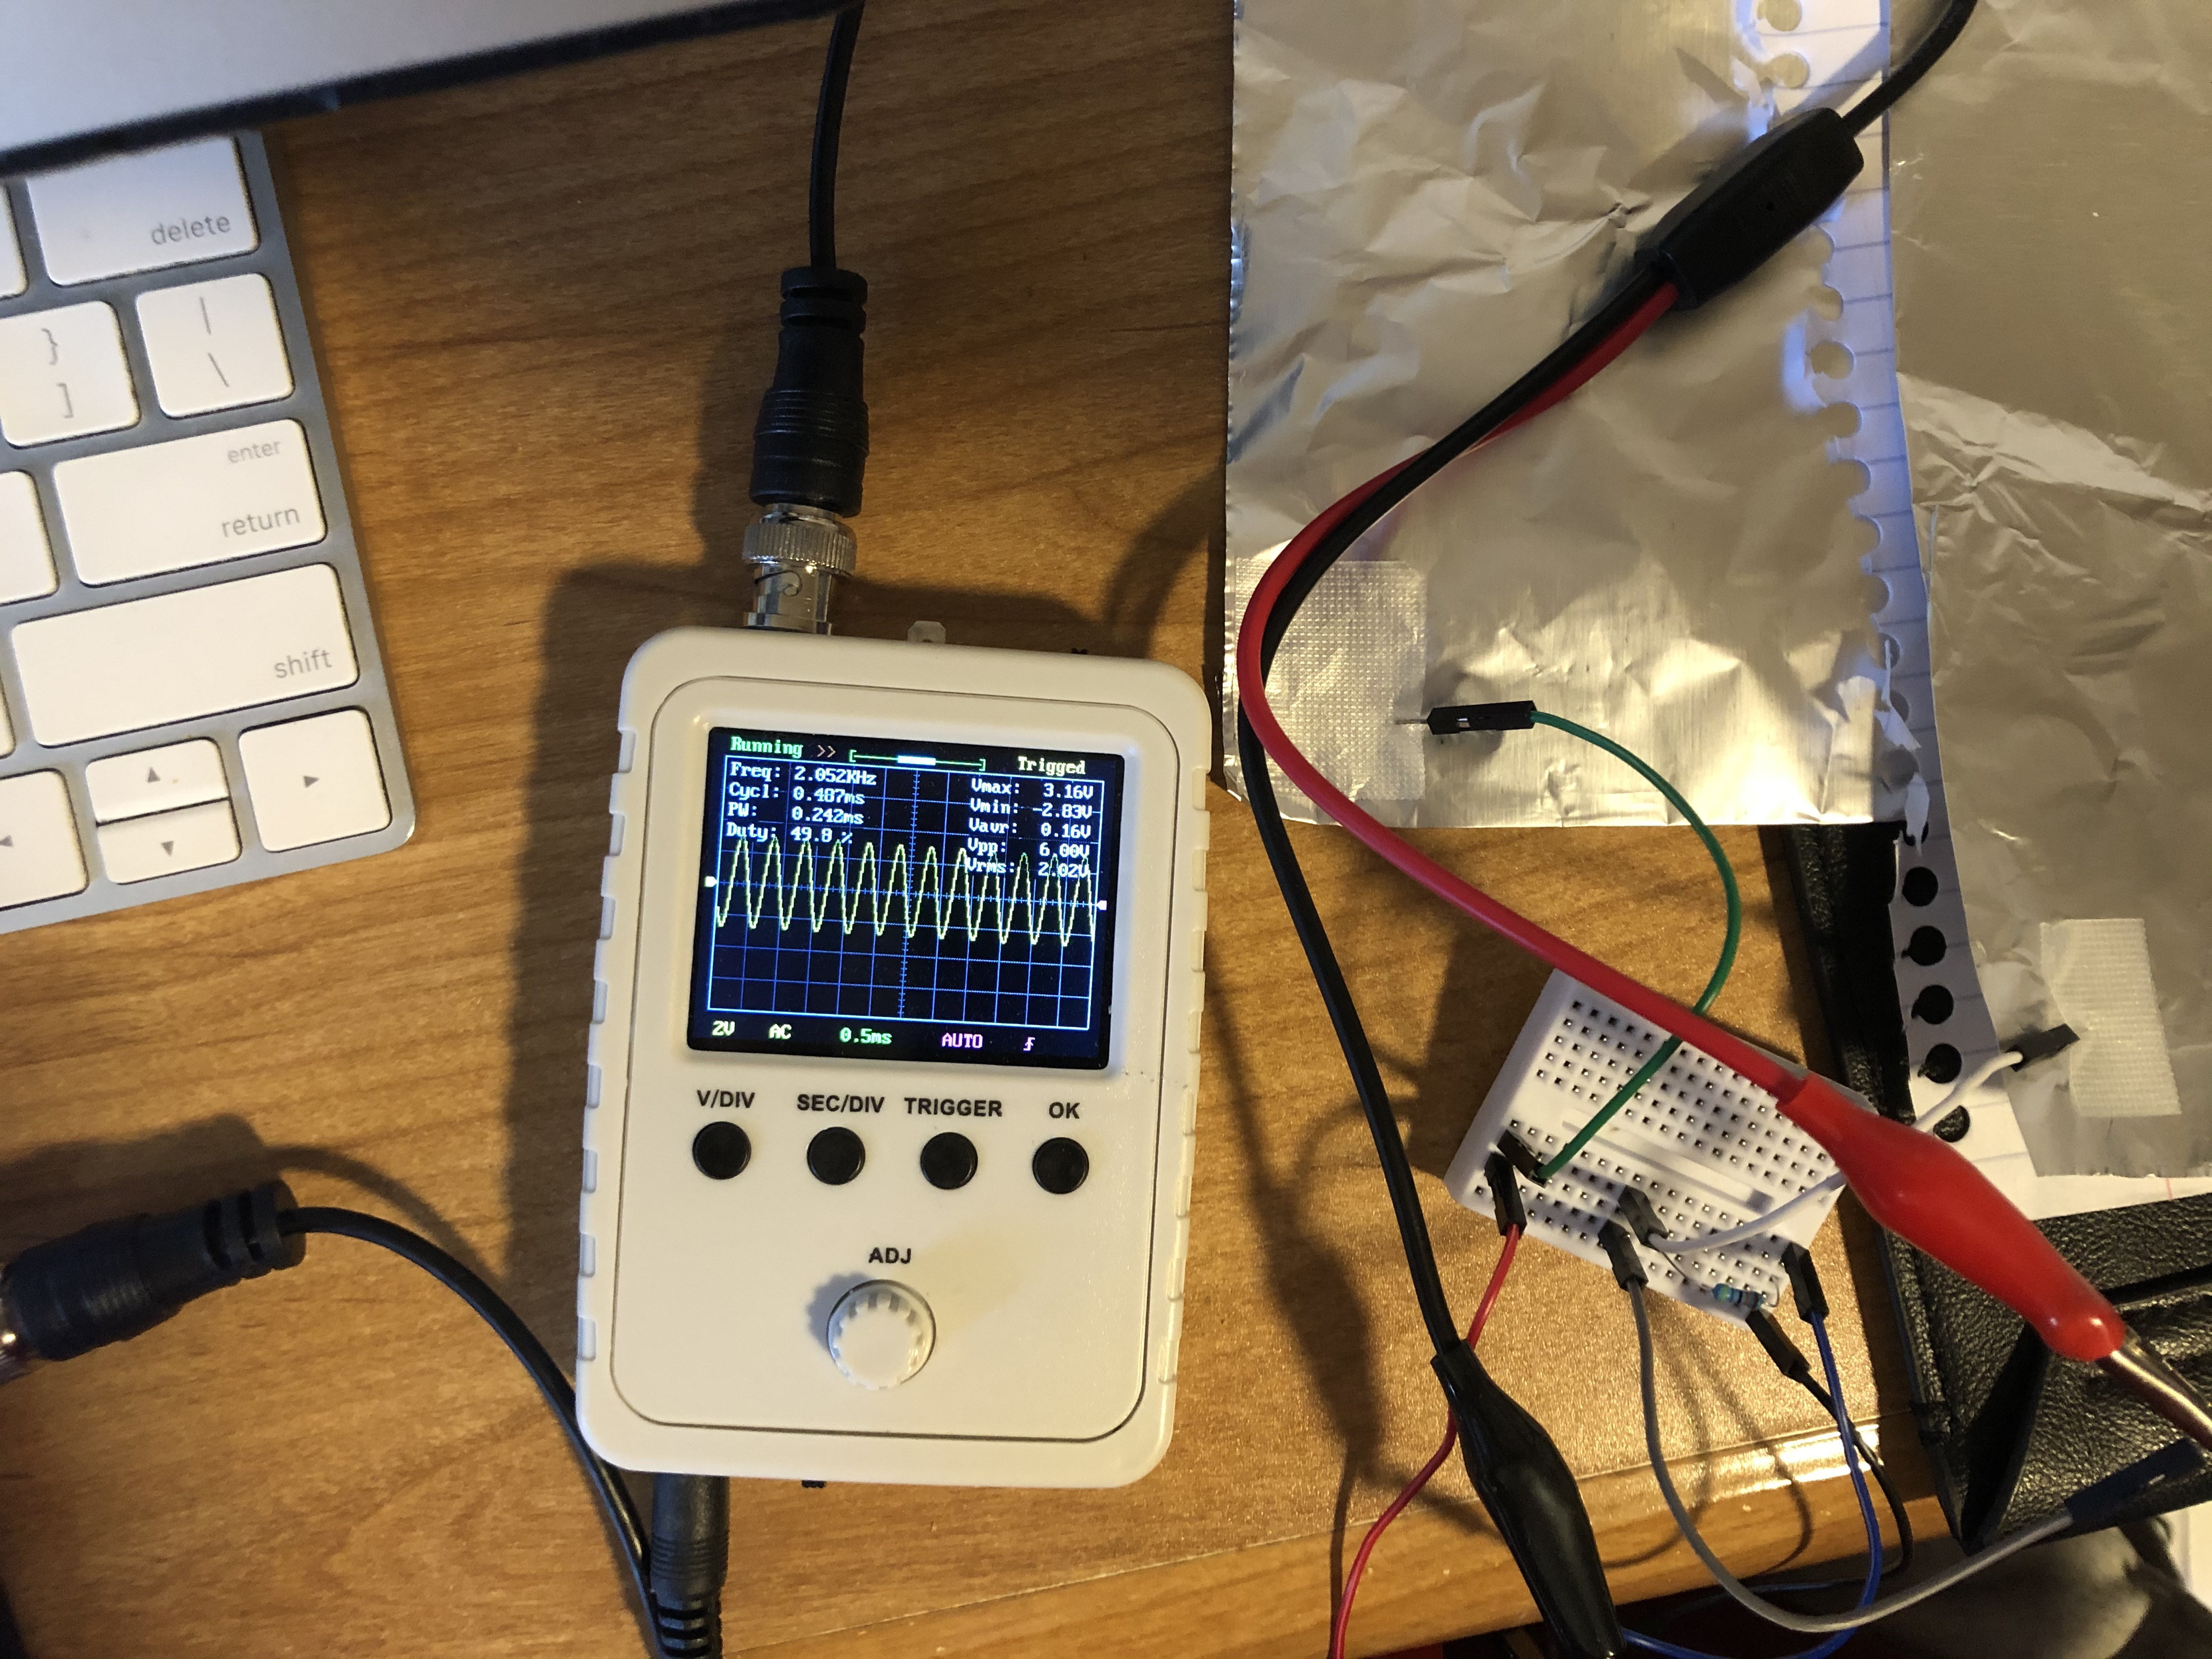
\includegraphics[scale=0.1]{2.jpeg}
  \subsection*{\(V_{RC}\)}
  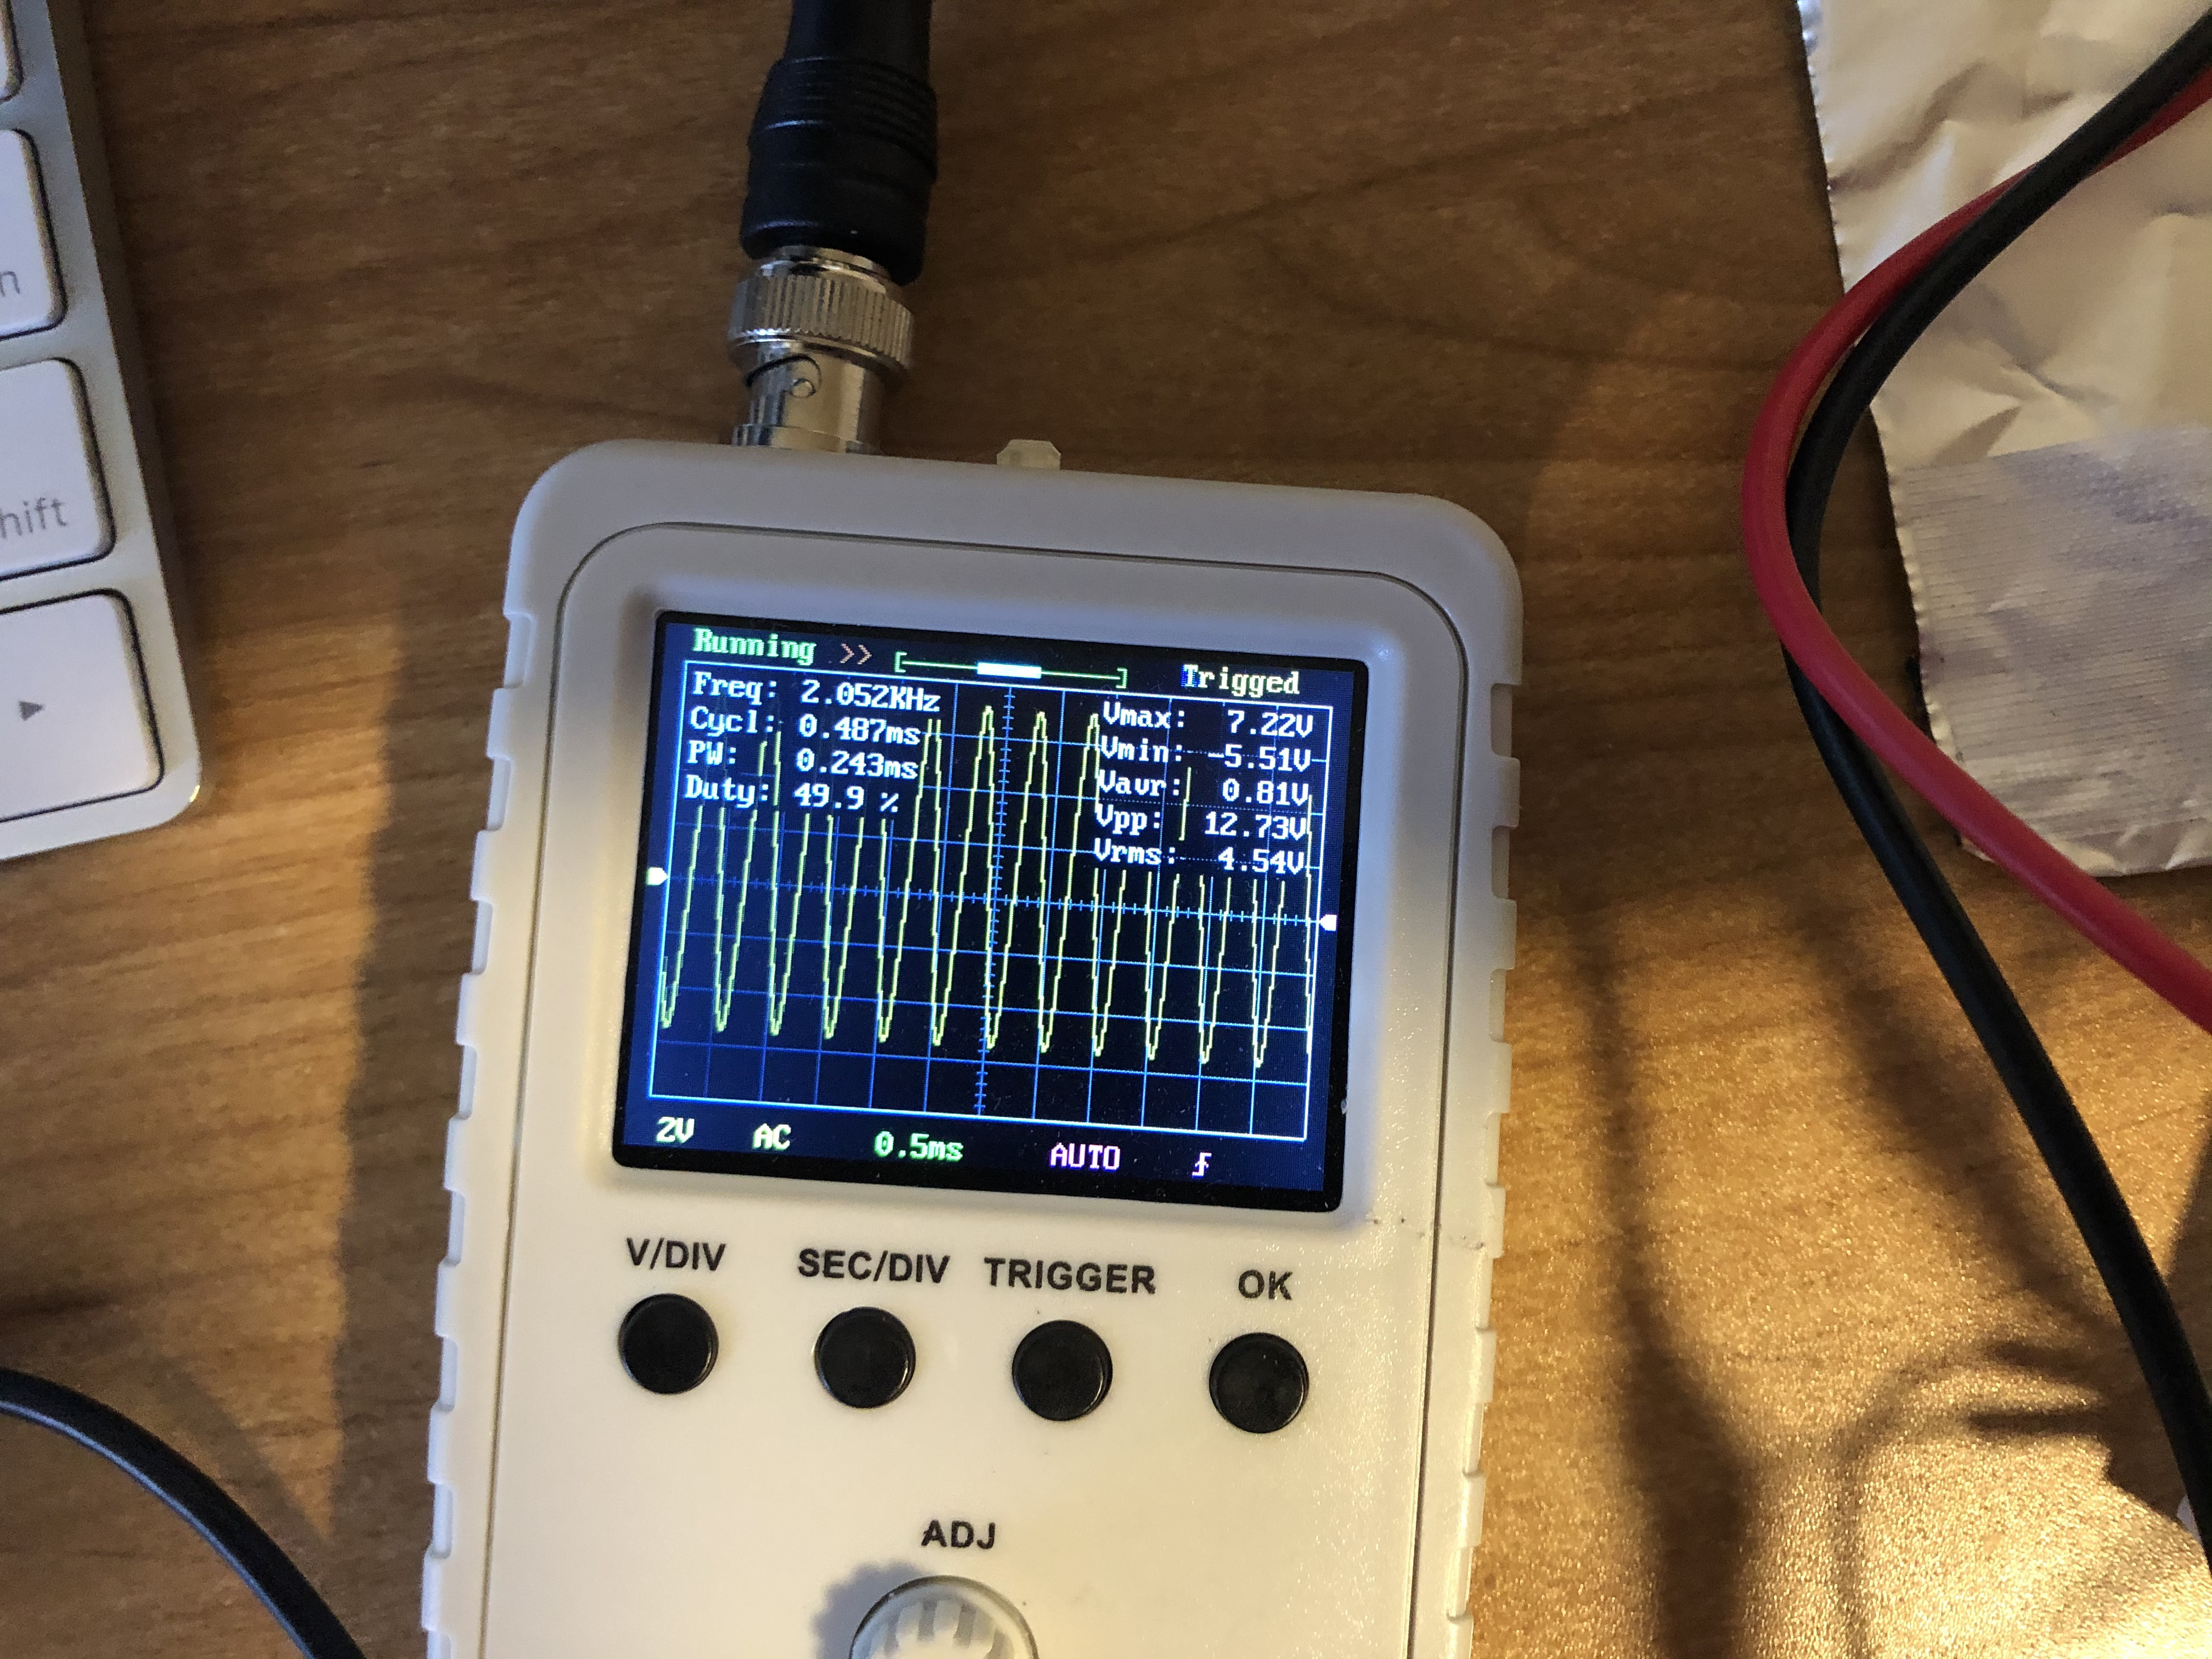
\includegraphics[scale=0.1]{1.jpeg}
\end{center}

\begin{center}
  \subsection*{Graph 1:}
  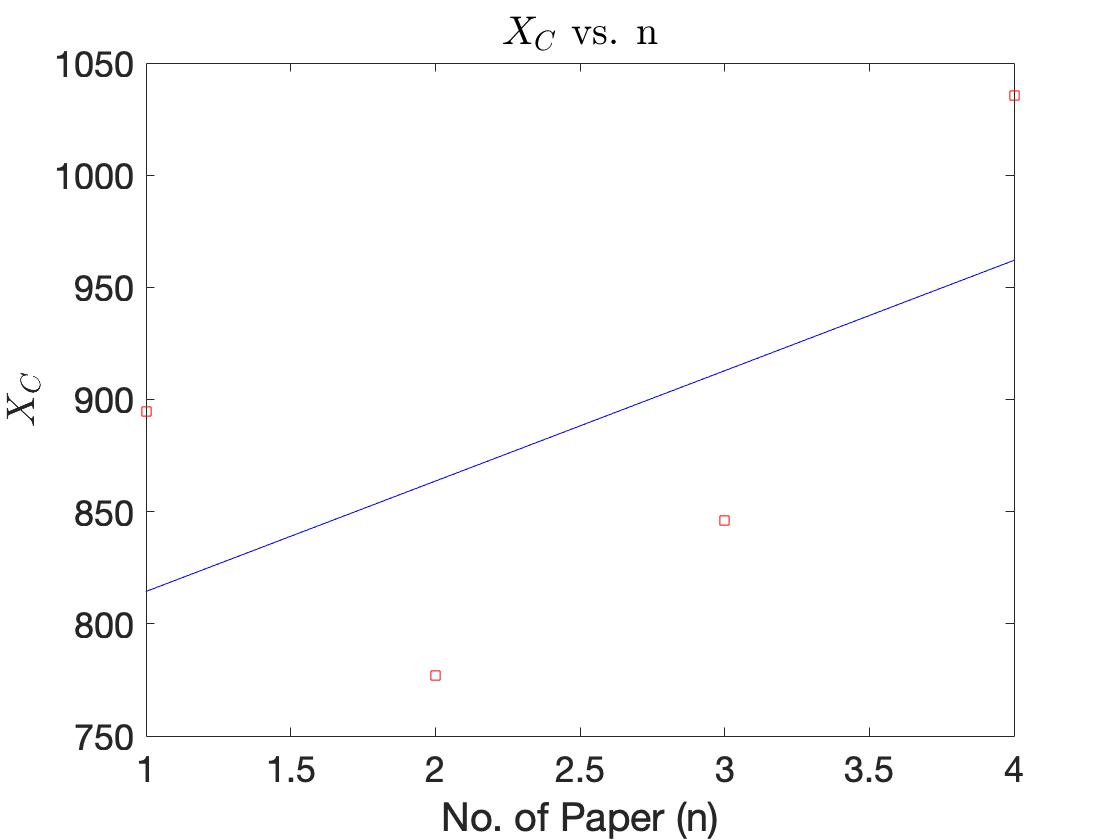
\includegraphics[scale=0.4]{graph1.jpg}
  \subsection*{Graph 2:}
  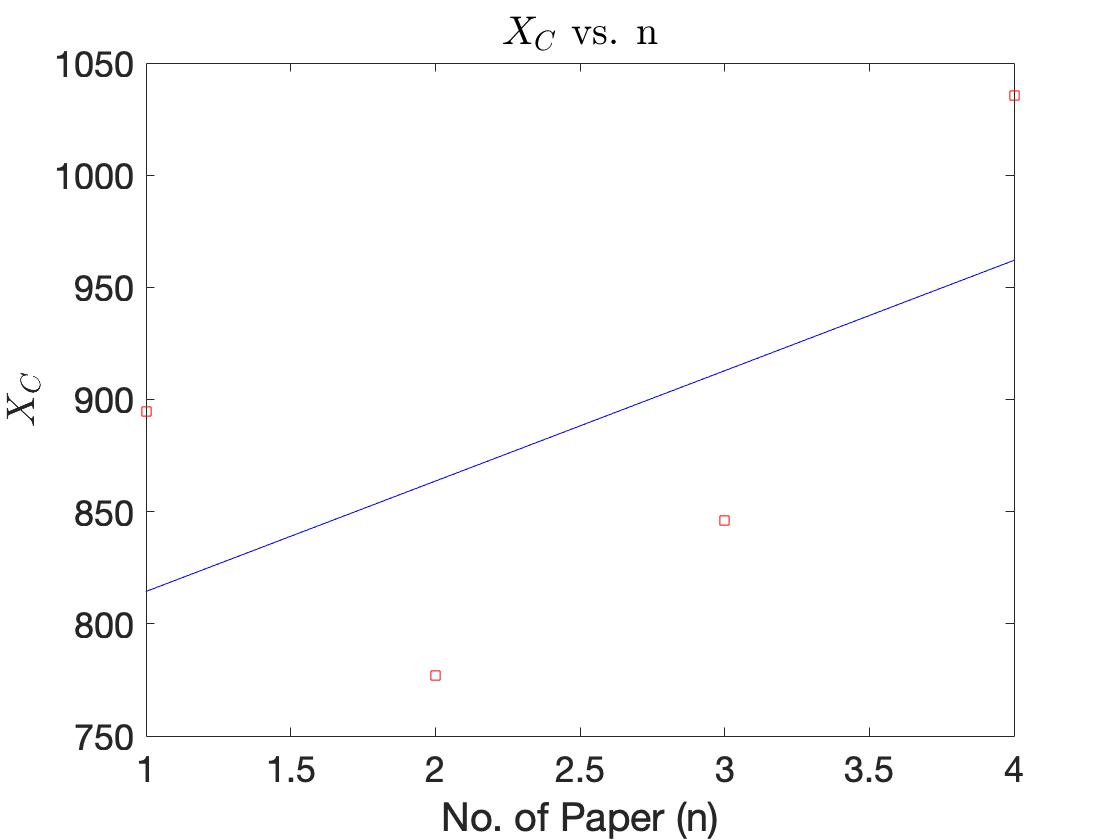
\includegraphics[scale=0.4]{graph2.jpg}
\end{center}

\begin{center}
  \begin{enumerate}
    \item What slope do you find for graph 2 and how does it compare to your expectation?
    \begin{itemize}
      \item
    \end{itemize}
    \item What do you think could cause the offset in the fit?
    \begin{itemize}
      \item Mostly from the aluminum foil
    \end{itemize}
  \end{enumerate}
\end{center}
\end{document}